\documentclass{llncs}
\usepackage[show]{ed}
\usepackage{wrapfig}
\usepackage{xspace}
\usepackage{graphicx}
\usepackage{stex-logo}
%\usepackage{lststex} debug that the gray is not solid
\usepackage{listings}
\definecolor{codegray}{rgb}{0.9,0.9,0.9}
\lstset{basicstyle=\sf,columns=fullflexible,backgroundcolor = \color{codegray}}
\lstset{numberstyle=\tiny}
\lstset{language={[LaTeX]TeX}}
\usepackage[style=alphabetic,hyperref=auto,defernumbers=true,backend=bibtex,firstinits=true,maxbibnames=9,maxcitenames=3,isbn=false]{biblatex}
\addbibresource{kwarcpubs.bib}
\addbibresource{extpubs.bib}
\addbibresource{kwarccrossrefs.bib}
\addbibresource{extcrossrefs.bib}
\usepackage[noabbrev]{cleveref}

% I do not want to annotate just yet.

\newcommand\ALeA{\textsf{ALeA}\xspace}
\newcommand\snify{\textsf{snify}\xspace}
\def\llangle{\langle\kern-.2em\langle}
\def\rrangle{\rangle\kern-.2em\rangle}

\title{Bulk Semantic Annotation with a Partially Known Knowledge Base}
\author{Michael Kohlhase, Jan Frederik Schaefer}
\institute{Computer Science, FAU Erlangen N\"urnberg, Germany}
\begin{document}
\maketitle
\begin{abstract}
tbw
\end{abstract}

\section{Introduction}
Arguably, dealing with large document collections is one of the key factors in the
knowledge-driven society and economy. There are currently two main contenders for machine
support in this area. Symbolic/logic-based technologies and sub-symbolic,
machine-learning-based AI, e.g.\ via LLMs or chatbots. They have complementary strengths
and challenges: Symbolic technologies offer precision and explainability out of the box,
but face scalability challenges because the prerequisite background knowledge has to be
(manually) formalized. ML-based approaches can be trained on all data of the Internet, but
face challenges in precision and explainability. In \cite{Ranta:atcp17},
Aarne Ranta matches these profiles to the notion of \textbf{producer tasks} -- i.e.\ tasks
where precision is key, but limited coverage ($10^{3\pm1}$ concepts) is OK;
e.g.\ for multi-language/variant manuals for very
expensive machines -- and \textbf{consumer tasks}, where coverage is key and
precision secondary; e.g.\ for consumer-grade machine translation like \textsf{Google translate}.

In this paper, we address tools that help attack the coverage problem in symbolic/semantic
approaches in practice. The producer task we use as a case study is that of adaptive
learning assistants for MINT subjects, concretely the \ALeA system \cite{BerBetChu:lssmkm23}.
\ALeA uses \sTeX \cite{MueKo:sdstex22,sTeX:github:on} -- a
variant of {\LaTeX} that allows to embed semantic annotations -- for knowledge
representation, and generates learner-adaptive learning objects instrumented with
learning-support interactions from that. The \textbf{\sTeX/\ALeA content commons}
\ednote{MK@MK: continue to describe the size and distribution, and
  authorship}\ednote{explain the \textbf{domain model} (the SMGloM) and the
  \textbf{formulation model} (cf. \cite{BerBetChu:lssmkm23}) in the commons and give their
  relative sizes.}

We contend that while education -- especially higher education -- as a whole is a
wide-coverage task for society education of individual learners in specific domains --
especially, if we want to tailor the educational offerings to said individual/domain -- is
a producer task, at least until ML-based methods reach the precision and explainability
required by the ethics of teaching.

\section{Semantic Authoring in a Content Commons}

Before we discuss semantic authoring in general, let us introduce a concrete example from
the \sTeX/\ALeA world. We will use it to sharpen our intuitions of the problems an issues
involved and to ground the solution we propose.

\subsection{Running Example: Annotating  ``Terminal''}
The main practical problem of annotating presentational {\LaTeX} course materials into
semantic documents that carry enough information to support meaningful learning support
services is to add semantic references to technical terms from the domain jargon.
% TODO: This the following better?
% With \sTeX, authors can add semantic references to technical terms,
% which enables straight-forward learning support services like
% showing the definition of a term, but also informs the system
% about the content/prerequisites of a learning object.
% Adding these references is a key practical problem when converting presentational {\LaTeX}
% course materials into semantic documents.
Take for instance a learning object like the paragraph in \cref{fig:lo}, where we want to annotate
the term ``terminal'' with the (semantic) concept of ``a goal state of a search
problem''. The latter can either be defined earlier in the course or in the domain model
(or both).



\begin{figure}[ht]\centering
  \fbox{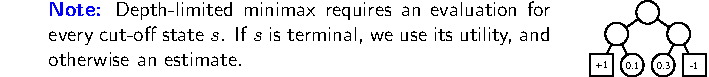
\includegraphics[width=10cm]{../img/minimax-remarks.pdf}}
  \caption{An annotated learning object from an AI lecture}\label{fig:lo}
\end{figure}

Concretely this is about converting the {\LaTeX} string
\begin{lstlisting}[numbers=left,firstnumber=3,
caption=The (unannotated) {\LaTeX} sources of \cref{fig:lo},label=lst:los]
\item \blue{Note:} Depth-limited minimax requires an evaluation for every
cut-off state $s$. If $s$ is terminal, we use its utility, and otherwise
an estimate.
\end{lstlisting}
into the (partially) annotated item:
\begin{lstlisting}[morekeywords={sr,importmodule},numbers=left,
caption=Annotating ``terminal'' in \cref{lst:los},label=lst:losa]
\importmodule[smglom/search]{mod?search-problem}
[...]
\item \blue{Note:} Depth-limited minimax requires an evaluation for every
cut-off state $s$. If $s$ is \sr{goal state}{terminal}, we use its utility,
and otherwise an estimate.
\end{lstlisting}
% Concretely, the author has to remember the module that introduces the concept
% of terminal states (\cref{fig:state-space}),
% the symbol name \lstinline|goal state|, annotate it with the
% \sTeX macro \lstinline[mathescape]|\sr{$\llangle symbol name \rrangle$}{$\llangle verbalization\rrangle$}|, and add the module import in the first line (unless it
% is already imported).
% If the symbol name and the desired verbalization coincide,
% the short-hand macro \lstinline|\sn| can be used (e.g. \lstinline|\sn{utility}|).

% In this case the symbol name happens to be the same as its English
% verbalization, otherwise we would have to use
% \lstinline[mathescape]|\sr{$\llangle symbol name\rrangle$}{state space}|.
The annotation refers to a definition in the domain model module shown in \cref{fig:state-space}.
The \lstinline|\definame| and \lstinline|\definiendum| in lines 5--6 introduce the \textbf{verbalizations} ``goal state'' and ``terminal state'' for the symbol \lstinline|search-problem?goal state| introduced by \lstinline|\symdecl*| declaration in line 3.

\begin{figure}[ht]\centering
  \fbox{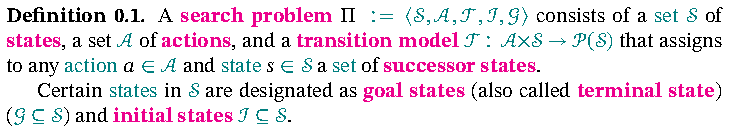
\includegraphics[width=12cm]{../img/search-problem.en.pdf}}
\begin{lstlisting}[morekeywords={definame,symdecl,definiendum},numbers=left]
\begin{smodule}[title=Search Problem]{search-problem}
[... some imports ...]
\symdecl*{goal state}
\begin{sdefinition}
  [...] Certain \sns{state} are [...] \definame[post=s]{goal state} [...]
  (also called \definiendum{goal state}{terminal states}).
\end{sdefinition}
\end{smodule}
\end{lstlisting}
  \caption{Simplified definition of ``goal state'' from the domain model}\label{fig:state-space}
\end{figure}

To annotate the string ``terminal'' in the learning object, the author has to be aware
that it is a technical term, that the module from \cref{fig:state-space} exists, know the
symbol name and its URL\ednote{path?}, and manage redundancy of the imports -- i.e. only
adding the \lstinline|\importmodule| directive if it is not already (recursively) implied
and possibly removing directives that become redundant by the new one.  At ca 150,000
words in a semester's words of lecture notes and ca. 10--15\%\ednote{can we actually
  measure this for AI?} of technical terms a rather daunting task.

\sTeX authoring is already supported by an VSCode IDE plugin \cite{sTeX-IDE:git} that
analyzes annotations on the fly, displays the underlying reference semantics, reports
errors and redundancies, and even offers a concept search interface.
But these features only support already annotated terms, so they do not solve the annotation problem above.

\subsection{Semantic Authoring as a Distinct Problem}

\begin{newpart}{MK: looking at the problem in general and compare it to the informal
    authoring and formal authoring problems e.g. programming in an IDE.}
We contend that semantic authoring is a problem that is distinct from traditional
(informal) authoring and authoring fully formal corpora (e.g. programs or formalizations),
while sharing some of the aspects of either.

In traditional authoring e.g. of a scientific article or a textbook, the domain model -- a
highly structured model of the domain of discourse -- is in the authors' heads, and is
partially verbalized e.g. in the preliminaries section or the main sections of the
respective article. The content is informal -- usually a natural language like english
augmented with technical jargon, formulae, tables, and diagrams -- and designed for
processing via the brain of a colleague or student -- in any case, a human who shares a
canonical part of the domain model with the authors.\ednote{MK: this shared domain model
  could be thought of as the informal content commons; hmmm, but maybe the literature is
  the content commons} Consequently a large part of the authoring problem lies in
predicting the state and extent of the domain model of the reader and creating text that
bridges the gap between the reader's domain model and the payload content of the article
-- the knowledge the article or textbook intends to impart -- ideally using the technical
vocabulary the reader is familiar with to reduce this gap. Tool support for traditional
authoring is minimal and usually restricted to spell/grammar-checkers and online thesauri
if we disregard LLM writing/formulation support for now.

In fully formal authoring e.g. for programming, the content commons is given formally in
the form of the libraries of the respective programming language, correspondingly the
authored content is also formal -- a program -- and intended for processing by a computer,
for which the formality is a prerequisite. Formal authoring is usually supported by an
integraded development environment (IDE) that makes use of the fully formal content and
offers services like semantic tab completion 

\ednote{talk about formalization in logic -- e.g. as theorem prover libraries as well}
\end{newpart}

  
\section{The \snify System}

The \snify\ednote{explain name? write as sn-ify?}
system (see \cite{stextools:git}) is a simple command-line tool
that creates a database of symbol-verbalization pairs, analyzes \sTeX source files,
and then steps through all word occurrences in the document that match a
verbalization in the database.
Matching is based on word stems using off-the-shelf stemmers, which allows us to
e.g.\ match ``utilities'' with ``utility''.
For each matched word, the user is presented with an annotation choice and
interactions that allow to fine-tune the wordwise annotation workflow. \Cref{fig:snify}
shows a typical situation.

\begin{figure}[ht]
  \setlength{\fboxsep}{0pt}
  \fbox{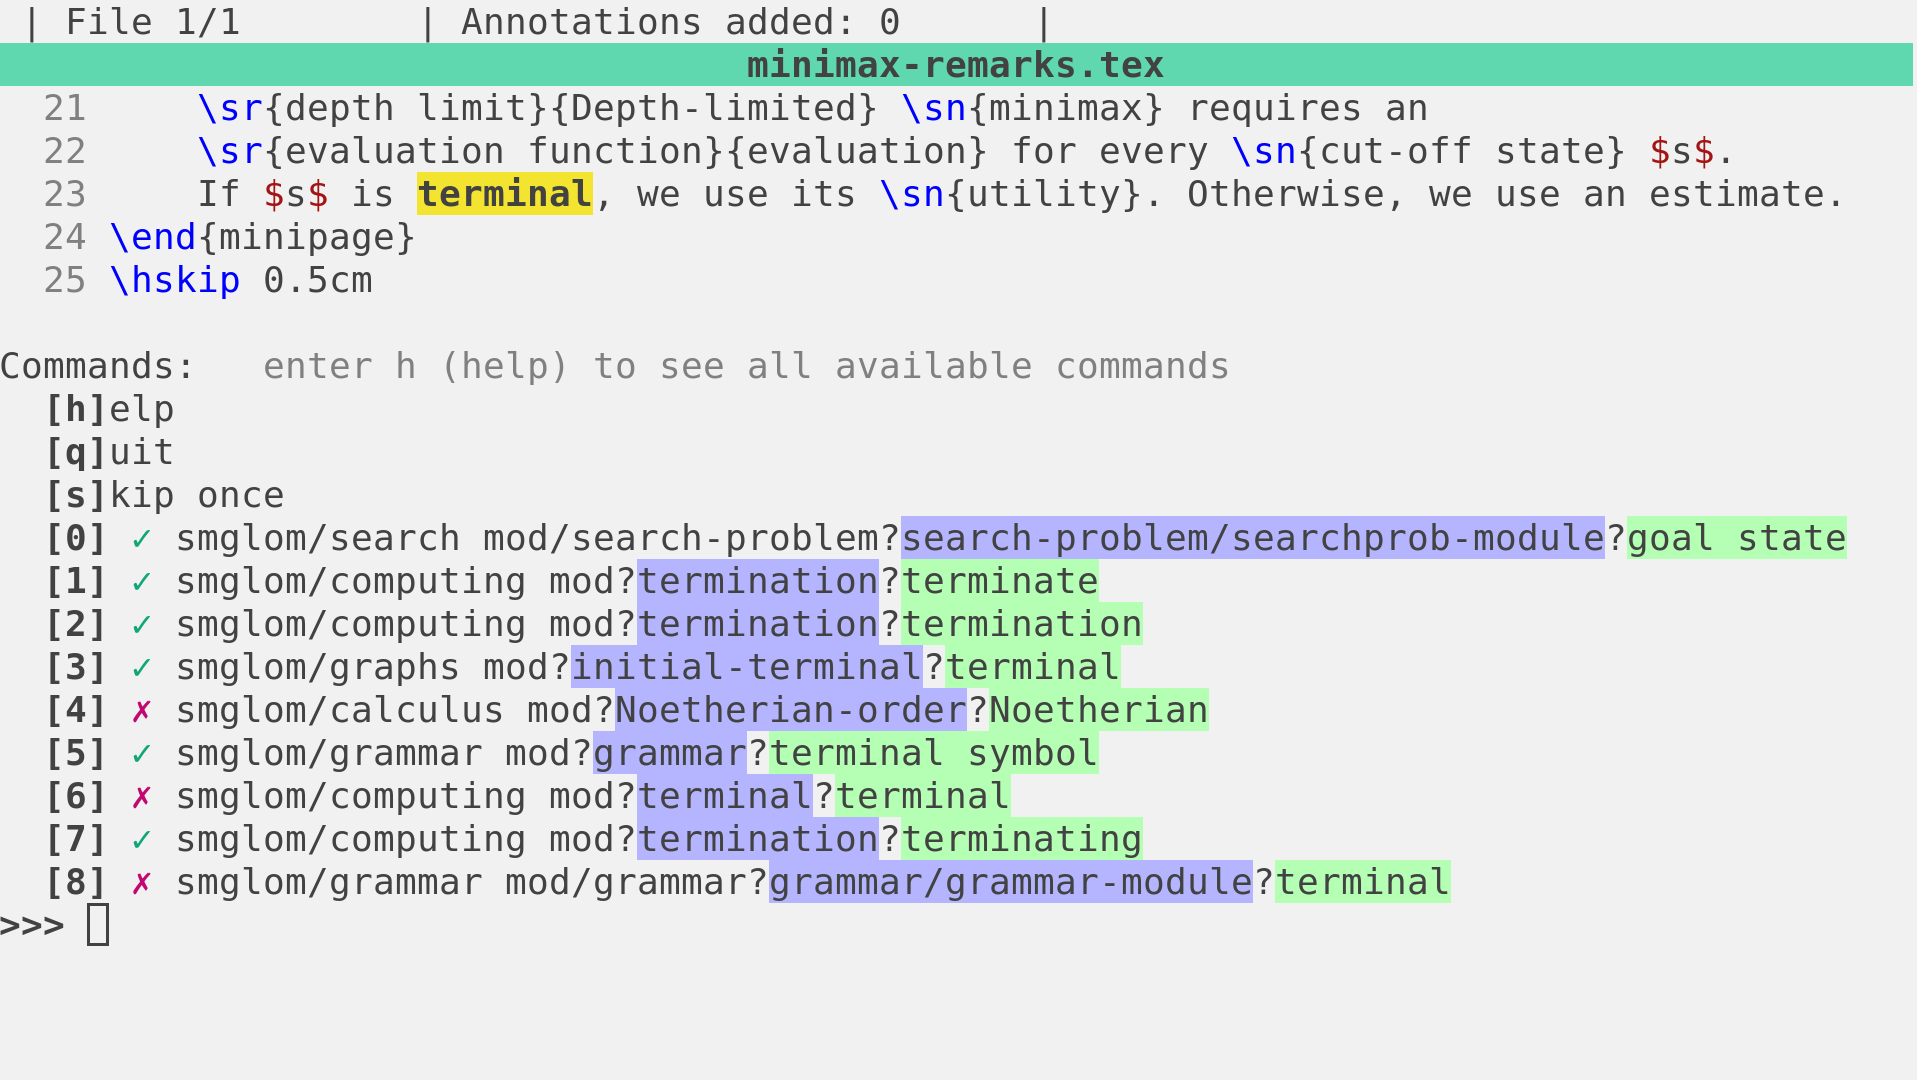
\includegraphics[width=12cm,trim={0 3cm 0 0},clip]{../img/snify}}
  \caption{\snify in Action: Annotating the word ``terminal''.}\label{fig:snify}
\end{figure}

The annotator can choose an annotation by typing the corresponding choice number,
in this case \lstinline|0|.
The little green check-mark indicates that the relevant module is already imported.
Otherwise \snify would offer the annotator the choice to import it -- if we are
in a module context -- or to add a \lstinline|\usemodule| directive, either in the
local environment or at the top-level.

To skip the word, the user can type \lstinline|s|,
\lstinline|s!| skips it until the end of the file, and \lstinline|S|
will skip it in future runs as well by appending a comment to the file.
There are numerous other commands, e.g.\ to adjust the selection,
search for alternative annotation targets,
or view the file introducing one of the choices.

\snify is usually called on a set of files -- e.g. in a directory or math archive -- which
together form a \textbf{session}, which can be interrupted and resumed without having to
re-do all the \lstinline|s| skips. Alternatively, \snify can be called e.g. on the top-level
lecture notes; then the session consists of all included files. Other productivity
features include a focus mode that can be used to only annotate a particular word in the
rest of the file, session, or the whole \sTeX/\ALeA corpus before resuming regular
annotation. This reduces the cognitive overhead from switching between different 
words and symbol lists.
% Of course the include management still needs to be done locally.

\section{Practical Evaluation}

In our experience, the step-through workflow for annotating term references for symbols
from the domain model is almost an order of magnitude more efficient than writing the
annotations and imports by hand, even for annotators who are familiar with the domain
model. For annotators unfamiliar with the domain model, the unassisted annotation task is
almost infeasible, and the average unfamiliarity naturally grows with the domain
model. The symbol disambiguation process -- on average a word induces $n$\ednote{MK@FS: we
  should try to measure this: for every verbalization (i.e. symbol/word pair) we should
  compute the ratio of those words with the same stem.} choices is still manageable,
requires considerable concentration and domain knowledge, but little knowledge of the
domain model flexiformalization.

The command-line interface is simple and responsive and gives all the necessary
information in a single glance if underlying shell area exceeds ca. $80\times 35$
characters. It is very much geared towards annotating existing documents with respect to a
relatively complete -- pre-existing -- domain model, and it seems unlikely that a more
sophisticated UI would add value for this use-case.

For less complete domain models we have to skip too many terms that should ultimately be
annotated and annotation efficiency suffers. This is currently the case for all
non-English languages in the \sTeX corpus we work with. Coverage in German is only about
half of that of English and we can already see the practical effects. We have also
experimented with a Slovene introductory math book, and it seems clear that apart from
having to introduce a Slovene stemmer\ednote{MK@FS: there is one for python at
  \url{https://repo.ijs.si/pboskoski/slo_stemmer}}, we would need to manually annotate all
definienda in the book before we can harvest the symbol/verbalization pairs which are a
prerequisite for annotation.

One practical problem with \snify that remains is that the system only harvests
symbol/verbalization pairs from \sTeX files on the local file system. This means that for
effective annotation users (have to) download the whole content commons and keep it
updated. Unfortunately, the current MMT-based MathHub knowledge management
API\ednote{intro this above} does not supply verbalization information. The iMMT-based
API~\cite{iMMT:on} currently under development will, so \snify will be able to request the
pairs for the remaining (non-local) content commons. If a pair is chosen in an annotation,
\snify can then automatically download the corresponding archive so that the annotated
file can be formattted with pdflatex or rusTeX locally.

Finally, the current interface is not well-suited for on-the-fly annotation while
authoring.  For that, the underlying information (the symbol/verbalization pairs harvested
from the domain model) can be integrated into any IDE. In fact we plan to do this for the
next version of the sTeX plugin for VSCode \cite{sTeX-IDE:git}.

\section{Conclusion}

In this paper we have presented the semantic authoring problem using the \sTeX corpus and
the adaptive learning assistant \ALeA as a concrete example. We have shown that it differs
from both classical authoring and formal authoring in terms of the necesssary system
support. As an example of specialized authoring support, we have presented \snify, a
command-line tool that bridges the gap between formal symbols in \sTeX and 

\snify is open source; the source and documentation are available from
\cite{stextools:git}.

In an earlier attempt to support semantic annotation in IDEs, we tried named-entity
recognition (NER) for classification of ``likely annotation candidate words''
\cite{hutterer:msc23}, however this classification was not precise enough in the
distinction in ``technical terms'' and ordinary English noun phrases and named entities --
the relevant task for annotation, and so made it impractical, especially, since it could
not enter the actual annotations and import directives automatically. But maybe using the
NER-based approach, after the \snify annotation process might change the trade-offs
involved. In any case, the overall workflow suggested by the NER-based approach --
especially after the verbalizations covered by the existing domain model\ednote{introduce
  in the definition above that the domain model is all definitions, not only in the
  smglom?} -- is geared towards adding modules and symbols -- the ones discovered by NER
-- to the domain model. 

\printbibliography
\end{document}

%%% Local Variables:
%%% mode: latex
%%% TeX-master: t
%%% End:

% LocalWords:  tbw Aarne Ranta homostem pre
